\chapter{Background}
\label{ch:background}

\section{Fixed-point iteration}
% TODO drop this?
% TODO define trial and result

Considering a function \(\varphi\colon M \to M\) which maps \(M\) to itself and a start point \(x_0 \in M\). The sequence \((x_k)_{k \in \mathbb{N}_0}\) generated by the fixed-point iteration is defined by \(x_{k+1} = \varphi(x_k)\) with \(k \in \mathbb{N}_0\).

The Banach fixed-point theorem guarantees that the sequence converges to the single fixed-point \(\varphi(x) = x\) if \(M\) is a complete metric space and \(\varphi\) is a contraction.

\section{DMFT}
% TODO quantum monte carlo?
% TODO second quantisation?

Dynamical mean-field theory (DMFT) is a method to determine the electronic structure of strongly correlated materials. It can be solved thourgh a self-consistency iteration shown in figure \ref{fig:dmft}.
It is basically a fixed-point iteration \(\varphi(x) = x\) with a very complicated, non-linear function \(\varphi\). The questions about existence and unambiguity have no general answer yet.

\begin{figure}[H]
    \centering
    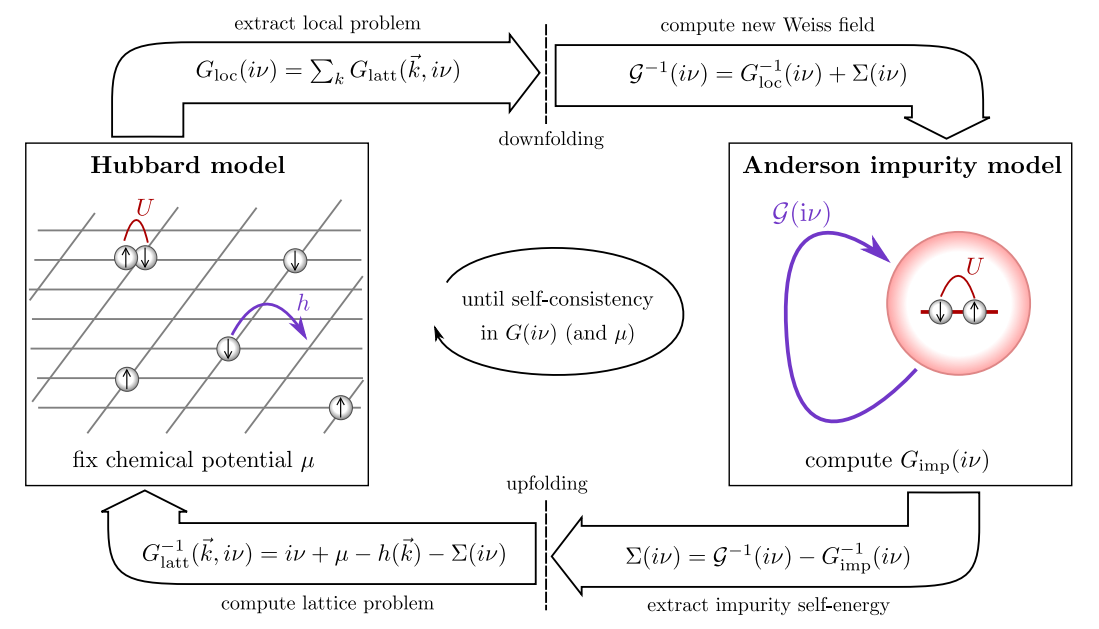
\includegraphics[width=1.0\textwidth]{figures/dmft.png}
    \caption{Self-consistency loop of dynamical mean field theory for a Hubbard-type model.}
    \label{fig:dmft}
\end{figure}

\section{Mixing}

Mixing is a technique to improve convergence for self-consistency iteration. The idea is to construct a more effective trial with more information than just the previous result. To be effective such a trial has to be closer to the true value which means we want to extrapolate in terms of iterations.

Probably the simplest approach would be the linear mixing \(\hat{x}_k = (1-\beta) x_k + \beta \varphi(x_k) = x_k + \beta (\varphi(x_k) - x_k)\), with the relaxation parameter \(\beta\).
For \(0 < \beta < 1\) we get an under-relaxation which slows down convergence in general but dampens systematic or statistical fluctualtions between iterations. If the self-consistency iterations diverge, the use of under-relaxation might help out.
For \(\beta > 1\) we get over-relaxation which has predictive behaviour and can speed up the convergence but it also amplifies errors and might result in divergence.

More complex mixing techniques would use multiple trials and results of the previous iterations and try to combine under-relaxation for robustness and prediction to increase the rate of convergence.

\section{DIIS}
% TODO least squares interpretation (svd?)

The direct inversion of the iterative subspace (DIIS), also known as Pulay mixing, is an extrapolation technique developed by Peter Pulay. His intention was to accelerate and stabelize the convergence of the Hartree-Fock self-consistent field method.

DIIS utilizes trials and results of multiple previous fixed-point iterations to construct a linear combination of them to extrapolate a new trial for the next iteration. The coefficients are determined by a least squares optimization.

% TODO duplication of previous section?
We consider a fixed-point problem \(g(x) = x\) with \(g\colon \mathbb{R}^N \to \mathbb{R}^N\). The form
\begin{equation} \label{eq:diis_linmix}
x_{k+1} = x_k + \beta f_k
\end{equation}
with the relaxation parameter \(\beta \in \mathbb{R}\) and the \(k\)th residual \(f_k = g(x_k) - x_k\), is a common approach to increase stability by under-relaxation with \(0 < \beta < 1\), or to increase the rate of convergence by over-relaxation with \(\beta > 1\). This technique is only using one trial and one result and might converge slowly.

Pulay's DIIS attempts to guess a better trial by using multiple previous trials and results. The method assumes that a good approximation of the true value can be obtained by a linear combination of the previous trials.
\begin{equation} \label{eq:diis_x}
\overline{x}_{k} = \sum_{j=0}^{m} c_j x_{k-j}
\end{equation}
where \(m\) is the number of previous trials to consider. We can also write this sum in terms of the true value \(x\) and an error vector \(e_{k} = x - x_{k}\).
\[\overline{x}_{k} = \sum_{j=0}^{m} c_j (x + e_{k-j}) = x \sum_{j=0}^{m} c_j + \sum_{j=0}^{m} c_j e_{k-j}\]
To get close to the real value \(x\) we set \(\sum_{j=0}^{m} c_j = 1\) and try to minimize the second term \(\sum_{j=0}^{m} c_j e_{k-j}\). Since we don't know the true value \(x\) we cannot know \(e_{k}\). Further, we approximate \(e_{k} \approx f_{k} = g(x_k) - x_k\).
\[\overline{f}_{k} = \sum_{j=0}^{m} c_j f_{k-j}\]
In order to minimize \(\overline{f}_{k}\) we use the \(l^2\)-norm.

One solution would be to use the Lagrange multiplier technique to satisfy the constraint \(\sum_{j=0}^{m} c_j = 1\) and minimize \(|\overline{f}_{k}|^2\).

Another is to rewrite \(\overline{f}_{k}\) and embed the constraint.
\begin{equation} \label{eq:diis_f2}
\overline{f}_{k} = f_k - \sum_{j=1}^{m} \gamma_j {\Delta f}_{k-m+j}
\end{equation}
with \({\Delta f}_{k} = f_k - f_{k-1}\).

We minimize \(|\overline{f}_{k}|^2\) by \((\gamma_k)\) and get the solution
\[\Gamma_k = (F_k^T F_k)^{-1} F_k^T f_k\]
with \(\Gamma_k = [\gamma_j]_{j=1..m}\) and \(F_k = [{\Delta f}_{k-m+j}]_{j=1..m}\).

Similar to \eqref{eq:diis_linmix} we can contruct a new trial with \eqref{eq:diis_x} and \eqref{eq:diis_f2}.
\begin{equation} \label{eq:diis_final}
x_{k+1} = \overline{x}_k + \beta \overline{f}_k = x_k + \beta f_k - (X_k + \beta F_k) (F_k^T F_k)^{-1} F_k^T f_k
\end{equation}

Variations of the DIIS method exist to further increase the rate of convergence and stability. The restarted Pulay method\cite{diis_restarted} and the periodic Pulay method\cite{diis_periodic} reset the state or use linear mixing inbetween to reduce side effects of DIIS.

